\section{Geração e distribuição de energia}


\begin{frame}{Geração de energia}
	\begin{block}{Introdução}
		\begin{itemize}
			\item Você já pensou em como é gerada a energia que utilizamos?
			\item Lembra do \textbf{potencial}, abordado na primeira aula?
			\item A \textit{geração de energia }é meramente a \textbf{conversão }entre dois tipos de energias.
			\item No Brasil, grande parte de nossa energia elétrica provem da \textbf{energia potencial gravitacional} da água:
			      \begin{enumerate}
				      \item\normalsize O fluxo de um rio é \textbf{represado} de forma a aumentar sua \textbf{altura}.
				      \item\normalsize Na \textbf{queda} dessa água há \textbf{pás}, que possuem gigantes \textbf{ímãs} acoplados.
				      \item\normalsize Esses ímãs \textbf{induzem} a eletricidade em \textbf{bobinas} que \textbf{alimentam a rede elétrica}.
			      \end{enumerate}
		\end{itemize}
	\end{block}
\end{frame}


\begin{frame}{Geração de energia}
	\centering
	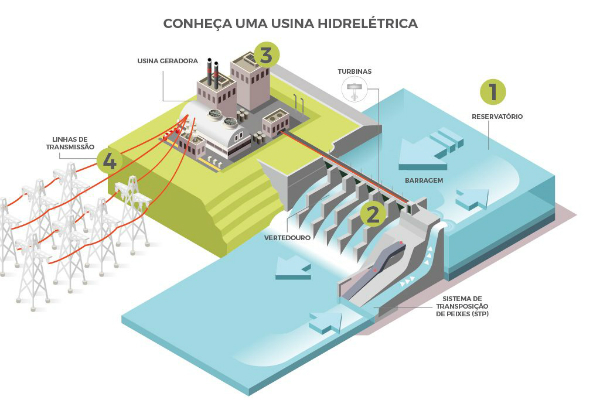
\includegraphics[width=1\linewidth]{Figuras/Ch03/fig1}
\end{frame}


\begin{frame}{Geração de energia}
	\centering
	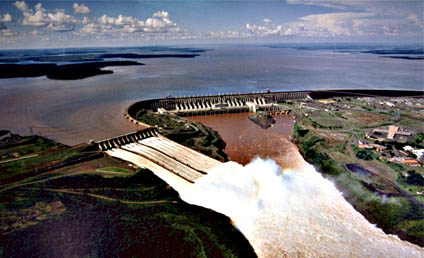
\includegraphics[width=1\linewidth]{Figuras/Ch03/fig2}
\end{frame}


\begin{frame}{Geração de energia}
	\begin{block}{Usinas}
		\begin{itemize}
			\item Nas hidrelétricas há, portanto, a conversão de \textbf{energia potencial} em \textbf{cinética} e, daí, em \textbf{elétrica}.
			\item A grande maioria das usinas se baseia nos \textbf{princípios indutivos} e, portanto, exige \textbf{movimento}.
			\item Nas \textbf{usinas nucleares}, por exemplo, a energia da \textbf{fissão dos átomos} (energia liberada quando os átomos se \textbf{quebram}) é convertida em \textbf{energia térmica}, que \textbf{aquece a água de um reservatório}.
			\item Esse vapor de água \textbf{movimenta} pás com ímãs que vão induzir tensão, de forma similar às hidrelétricas.
		\end{itemize}
	\end{block}
\end{frame}


\begin{frame}{Geração de energia}
	\centering
	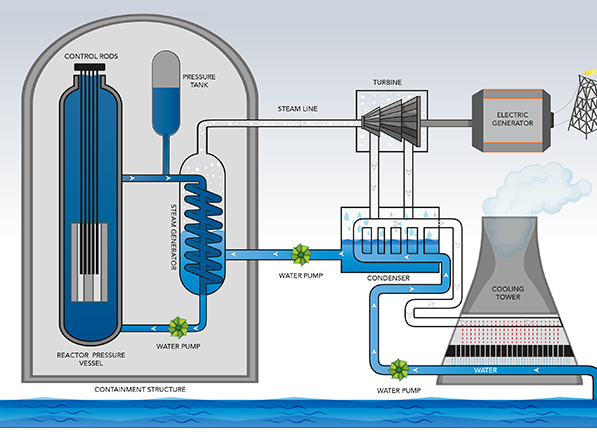
\includegraphics[width=0.9\linewidth]{Figuras/Ch03/fig3}
\end{frame}


\begin{frame}{Transmissão de energia}
	\begin{block}{Introdução}
		\begin{itemize}
			\item Da mesma forma, a \textbf{transmissão de energia} é algo \textbf{essencial} nesse processo.
			\item Não é viável gerar a energia que usamos em casa \textbf{individualmente}, pois os equipamentos são muito \textbf{caros} e de \textbf{difícil manutenção}.
			\item As alternativas \textbf{renováveis} também apresentam \textbf{problemas}, sejam eles de \textbf{custo} ou de \textbf{escala}.
			\item Os \textbf{painéis solares}, por exemplo, custam \textbf{caro}, e só funcionam \textbf{durante o dia}, e as \textbf{baterias} disponíveis hoje em dia são muito \textbf{caras}, \textbf{grandes}, e \textbf{limitadas}.
			\item Se juntássemos \textbf{todas} as baterias do \textbf{mundo}, conseguiríamos continuar usando nossos eletrodomésticos por, aproximadamente, \textbf{oito minutos}.
		\end{itemize}
	\end{block}
\end{frame}


\begin{frame}{Transmissão de energia}
	\begin{block}{Motivação}
		\begin{itemize}
			\item Dessa forma são necessárias alternativas de \textbf{transmissão de energia} gerada em grande escala para \textbf{todo o território nacional}.
			\item Devemos retomar os \textbf{fundamentos} de eletricidade discutidos na primeira aula, novamente.
			\item Quando falamos em \textbf{resistência}, podemos associar o \textbf{valor da resistência} de um condutor às suas características, como \textbf{comprimento} e \textbf{grossura} (bitola), além da \textbf{característica do próprio material}.
			\item Vamos retomar também as analogias com dutos, por onde passam fluidos.
		\end{itemize}
	\end{block}
\end{frame}


\begin{frame}{Transmissão de energia}
	\begin{block}{Noções básicas}
		\begin{itemize}
			\item Imagine dois tipos diferentes de dutos, um de \textbf{plástico rugoso} e outro de \textbf{metal polido}. Qual apresentará \textbf{menos resistência para a passagem de água}?
		\end{itemize}
	\end{block}

	\medskip

	\begin{minipage}{0.49\linewidth}
		\centering
		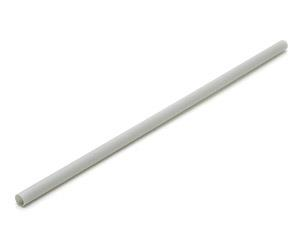
\includegraphics[width=\linewidth]{Figuras/Ch03/fig4}
	\end{minipage}
	\hfill
	\begin{minipage}{0.49\linewidth}
		\centering
		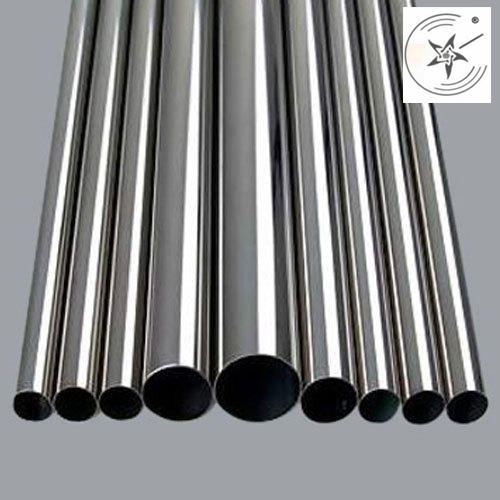
\includegraphics[width=\linewidth]{Figuras/Ch03/fig5}
	\end{minipage}

\end{frame}


\begin{frame}{Transmissão de energia}
	\begin{block}{Noções básicas}
		\begin{itemize}
			\item Agora pense na diferença de \textbf{grossura} e \textbf{comprimento} entre os tubos: por qual você acha que a água fluirá \textbf{mais facilmente}?
		\end{itemize}
	\end{block}

	\bigskip

	\begin{minipage}{0.49\linewidth}
		\centering
		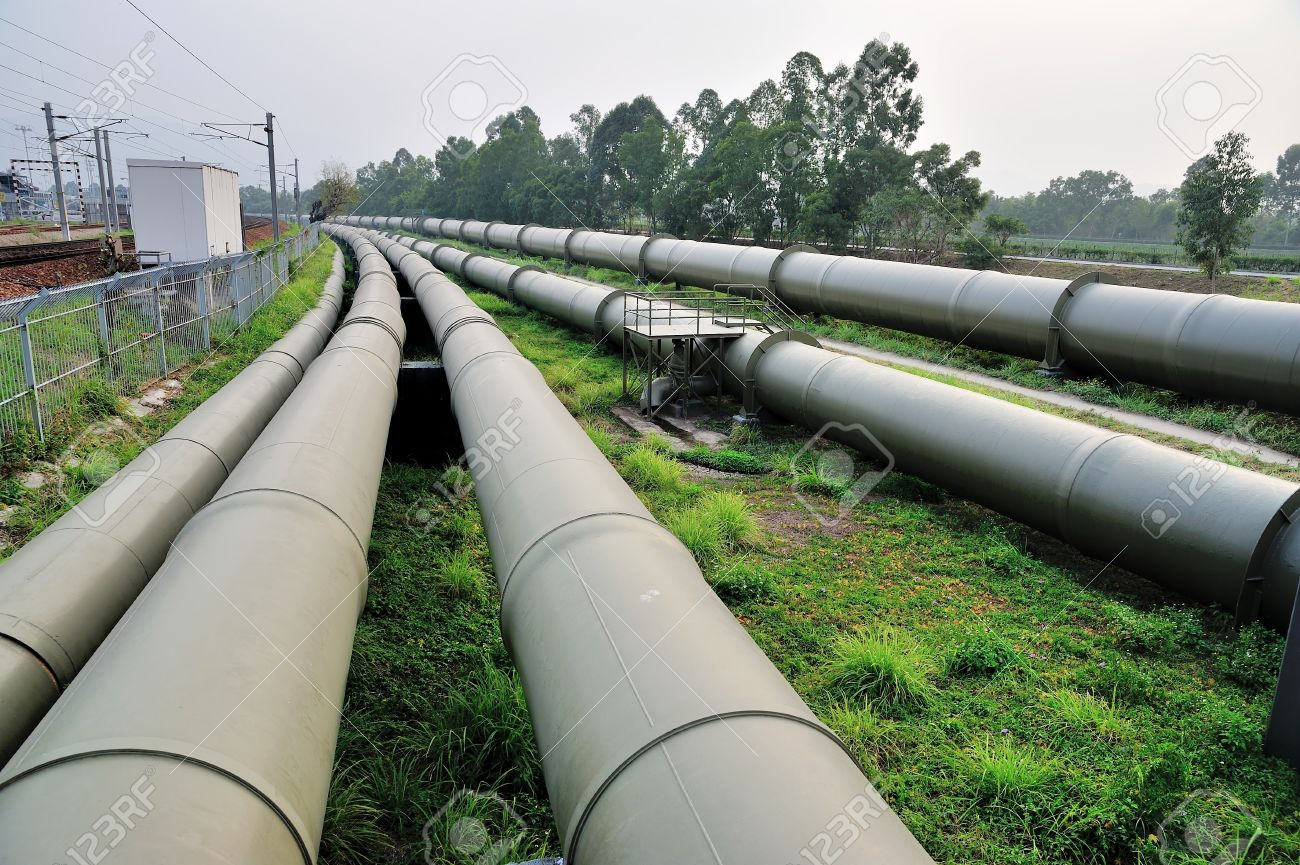
\includegraphics[width=\linewidth]{Figuras/Ch03/fig6}
	\end{minipage}
	\hfill
	\begin{minipage}{0.49\linewidth}
		\centering
		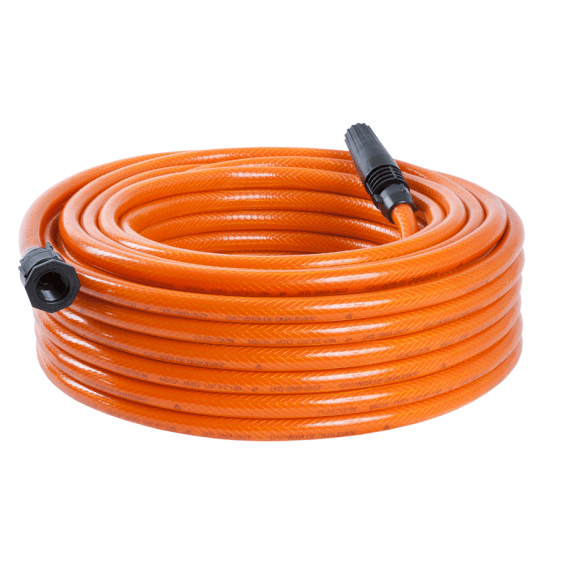
\includegraphics[width=\linewidth]{Figuras/Ch03/fig7}
	\end{minipage}

\end{frame}


\begin{frame}{Transmissão de energia}
	\begin{block}{Conclusões parciais}
		\begin{itemize}
			\item Podemos notar que a água flui \textbf{mais facilmente} quando posta num duto \textbf{largo}, \textbf{liso} e \textbf{curto} e, portanto, a resistência oferecida pelo duto é \textbf{proporcional ao seu comprimento} $ \bm{l} $, \textbf{proporcional à uma constante do material} $ \bm{\rho} $ e \textbf{inversamente proporcional à sua área} $ \bm{A} $, daí temos:\[ \boxed{R=\rho\dfrac{l}{A}} \]
			\item Utilizando esse raciocínio, por analogia, a \textbf{resistência elétrica} é dada \textbf{pela mesma fórmula}, mantidas as \textbf{peculiaridades} de cada grandeza física.
		\end{itemize}
	\end{block}
\end{frame}


\begin{frame}{Transmissão de energia}
	\begin{block}{Motivação}
		\begin{itemize}
			\item Agora, imagine um \textbf{fio gigante}, ligando o \textbf{sul} do Brasil, onde fica a usina de \textbf{Itaipu}, a uma grande cidade do \textbf{nordeste}, como \textbf{Fortaleza} ou \textbf{Natal}: \textbf{cerca de \SI{4200}{\kilo\meter} de fio!}
		\end{itemize}
	\end{block}

	\centering
	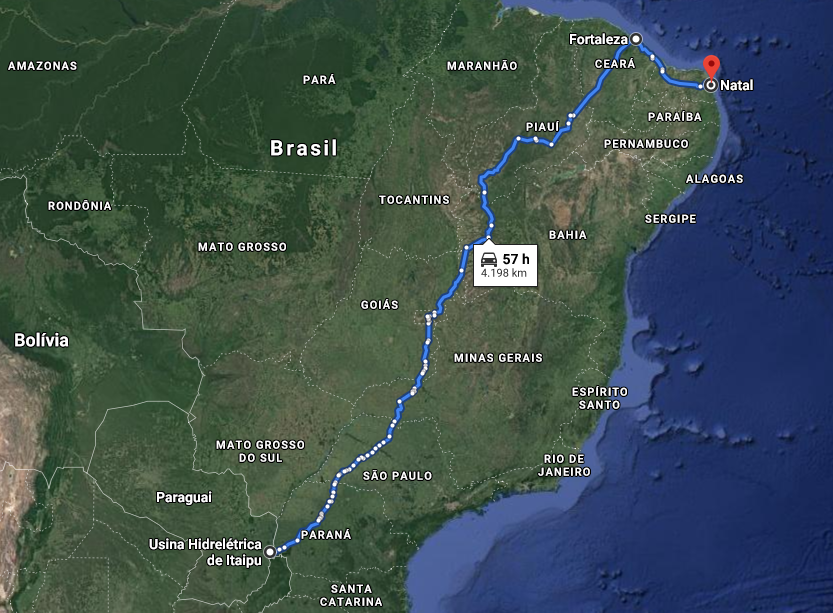
\includegraphics[height=0.6\textheight]{Figuras/Ch03/fig8}

\end{frame}


%\begin{frame}{Transmissão de energia}
%	\begin{block}{Motivação}
%		\begin{itemize}
%			\item Um dos metais condutores mais comuns que utilizamos é o cobre, que se encontra em praticamente toda instalação elétrica, porém nessas instalações é utilizada a prata, que possui resistividade ainda menor.
%			\item Se utilizarmos a resistividade da prata (conforme tabela abaixo), para efeito de cálculo, e a bitola parametrizada para transmissão a longas distâncias no Brasil (\SI{185}{\milli\meter\squared}), teremos $ \approx \SI{360}{\ohm} $ no percurso indicado.
%		\end{itemize}
%	\end{block}
%
%	\centering
%	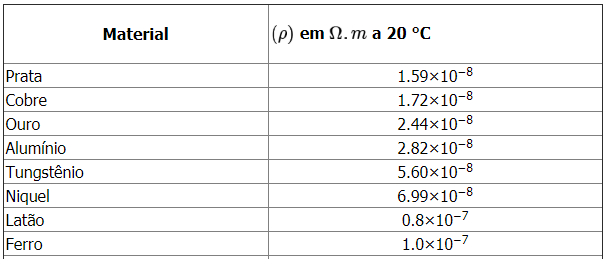
\includegraphics[width=0.7\linewidth]{Figuras/Ch03/fig9}
%	
%\end{frame}


\begin{frame}{Transmissão de energia}
	\begin{block}{Motivação}
		\begin{itemize}
			\item Imagine que transmitíssemos \textbf{\SI{127}{\volt}} nas linhas de tensão brasileiras para \textbf{território nacional}. No Ceará há um consumo de $ \approx \SI{4.129}{\giga\watt\hour} $ por ano, somente para uso \textbf{residencial}.
			\item Isso nos dá uma média de \SI{471347}{\watt} no condutor, com uma corrente igual à \SI{3711.4}{\ampere}.
			\item Pela tabela de corrente máxima do condutor (bitola padronizada de \SI{185}{\milli\meter\squared}), nota-se que esse aceitaria \textbf{no máximo \SI{280}{\ampere}}.
			\item Quando um fio \textbf{ultrapassa} a sua capacidade de \textbf{corrente} (e, portanto, de \textbf{potência}), ele começa a \textbf{derreter}, pois \textbf{precisa transferir a energia que flui nele} de alguma forma, e como \textbf{não consegue}, começa a se \textbf{aquecer demais}.
		\end{itemize}
	\end{block}

	%	\centering
	%	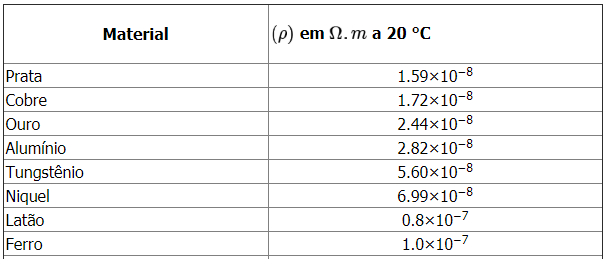
\includegraphics[width=0.7\linewidth]{Figuras/Ch03/fig9}

\end{frame}


\begin{frame}{Transmissão de energia}
	\begin{block}{Motivação}
		\begin{itemize}
			\item Um dos metais condutores \textbf{mais comuns} que utilizamos é o \textbf{cobre}, que se encontra em praticamente \textbf{toda instalação elétrica}, porém nas instalações para transmissão é utilizada a \textbf{prata}, que possui resistividade \textbf{ainda menor}.
		\end{itemize}
	\end{block}

	\centering

	\begin{tabular}{lc}
		\toprule
		\makecell[c]{Material} & $ \rho $ (\si{\ohm\meter} a \SI{20}{\degreeCelsius}) \\ \midrule
		Prata                  & \num{1.59e-8}                                        \\
		Cobre                  & \num{1.72e-8}                                        \\
		Ouro                   & \num{2.44e-8}                                        \\
		Alumínio               & \num{2.82e-8}                                        \\
		Tungstênio             & \num{5.60e-8}                                        \\
		Níquel                 & \num{6.99e-8}                                        \\
		Latão                  & \num{0.8e-7}                                         \\
		Ferro                  & \num{1.0e-7}                                         \\
		...                    & ...                                                  \\ \bottomrule
	\end{tabular}
	%		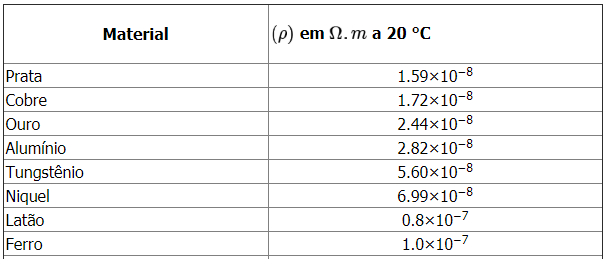
\includegraphics[width=0.9\linewidth]{Figuras/Ch03/fig9}

\end{frame}


\begin{frame}{Transmissão de energia}
	\begin{block}{Motivação}
		\begin{itemize}
			\item Além disso, utiliza-se uma bitola \textbf{bem mais grossa} do que aquela que temos em \textbf{casa}, para possibilitar correntes \textbf{bem altas}.
		\end{itemize}
	\end{block}

	\begin{minipage}{0.49\linewidth}
		\centering
		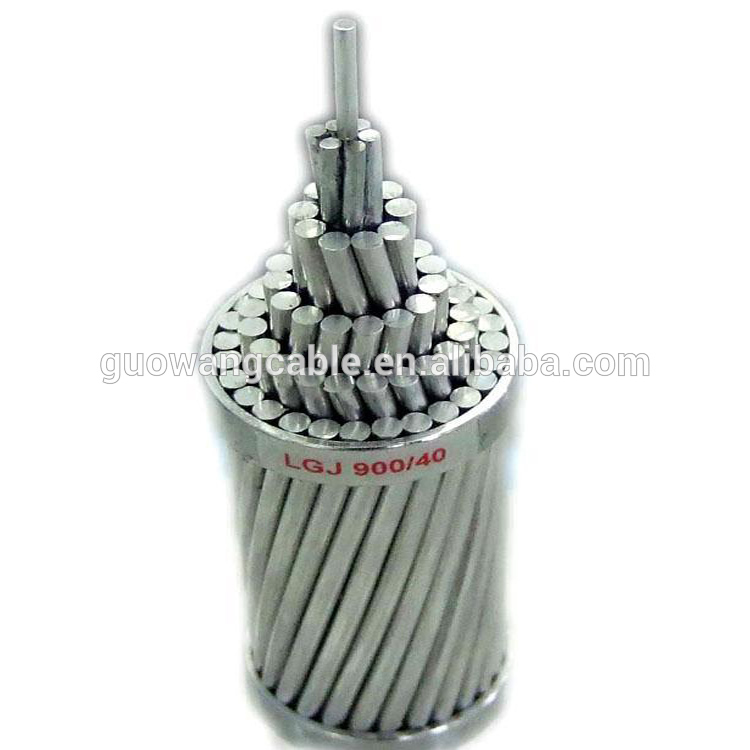
\includegraphics[width=\linewidth]{Figuras/Ch03/fig10}
	\end{minipage}
	\hfill
	\begin{minipage}{0.49\linewidth}
		\centering
		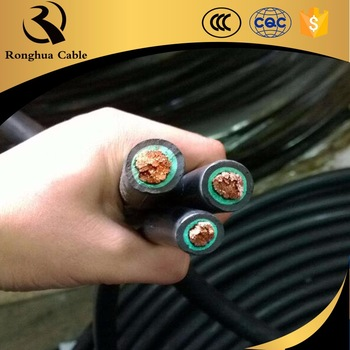
\includegraphics[width=\linewidth]{Figuras/Ch03/fig11}
	\end{minipage}

\end{frame}


\begin{frame}{Transmissão de energia}
	\begin{block}{Motivação}
		\begin{itemize}
			\item Porém, mesmo assim, \textbf{não conseguiríamos} suprir toda a demanda no Ceará utilizando as instalações de \textbf{baixa tensão}.
			\item Até mesmo com \textbf{\SI{220}{\volt}}, teríamos \SI{2142.5}{\ampere} no fio de alta tensão.
			\item Utilizando um sistema de \textbf{tensão alternada} com três fases, temos \textbf{\SI{714.2}{\ampere} por fase}, mas \textbf{ainda não dá} pra suprir a demanda residencial.
			\item Além disso, \textbf{uma alta potência dissipada diminui drasticamente o potencial do fio}, que, \textbf{mesmo possuindo uma resistência ínfima} ($ \approx \SI{360}{\ohm} $ no caso considerado), \textbf{acaba se tornando considerável à grandes distâncias}.
		\end{itemize}
	\end{block}

\end{frame}


\begin{frame}{Transmissão de energia}
	\begin{block}{Motivação}
		\begin{itemize}
			\item Se utilizarmos \textbf{tensões mais altas}, no entanto, é possível \textbf{suprir a demanda do estado inteiro}. Até mesmo a \textbf{demanda industrial}, que é a \textbf{maior} percentualmente.
			\item E, dessa forma, pode-se, inclusive, suprir \textbf{toda a demanda do país}.
			\item No geral, a tensão nas linhas de transmissão chega aos \textbf{\SI{230}{\kilo\volt}}!
			\item Porém, o grande problema disso é que, altas tensões são \textbf{potencialmente mortais} para seres humanos. Além disso, esses fios devem ficar bem separados, pois essas tensões são capazes de ionizar o ar, formando os famosos \textbf{arcos elétricos}.
			\item Daí a importância dos \textbf{transformadores}.
		\end{itemize}
	\end{block}

\end{frame}


\begin{frame}{Transmissão de energia}

	\centering
	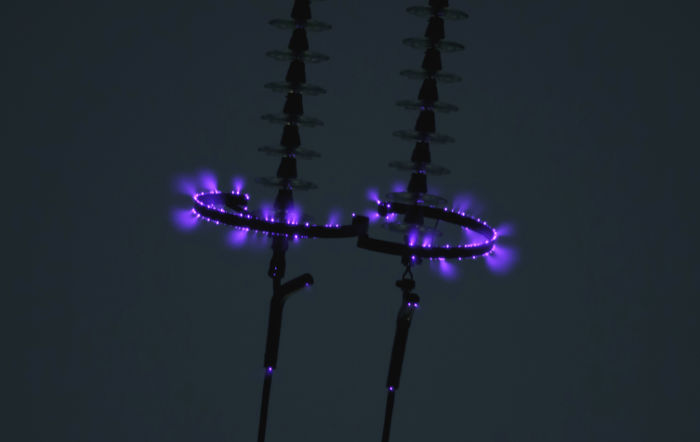
\includegraphics[width=\linewidth]{Figuras/Ch03/fig12}
\end{frame}


\begin{frame}{Transmissão de energia}
	\begin{block}{Transformadores e subestações}
		\begin{itemize}
			\item Nas \textbf{grandes distâncias} presentes na transmissão da energia para \textbf{distribuição nacional}, é essencial o uso de \textit{estações}, para que a energia elétrica seja \textit{tratada}.
			\item Uma \textit{subestação} é uma \textbf{instalação elétrica} de \textbf{alta potência}, contendo equipamentos para \textbf{transmissão }e \textbf{distribuição }de energia elétrica, além de equipamentos de \textbf{proteção} e \textbf{controle}.
			\item Trata-se de um ponto onde o \textbf{fluxo energético} pode ser \textbf{direcionado} e \textbf{controlado}, transformando os \textbf{níveis de tensão }e funcionando como \textbf{ponto de entrega }para \textbf{consumidores industriais}.
			\item Durante o percurso entre as usinas e as cidades, a eletricidade passa por diversas subestações, onde os \textbf{transformadores aumentam} ou \textbf{diminuem }a sua tensão.
		\end{itemize}
	\end{block}

\end{frame}


\begin{frame}{Transmissão de energia}
	\begin{block}{Transformadores e subestações}
		\begin{itemize}
			\item Ao \textbf{elevar a tensão }elétrica no \textbf{início da transmissão}, os transformadores \textbf{evitam }a\textbf{ perda excessiva de energia }ao longo do percurso.
			\item Ao \textbf{rebaixarem a tensão }elétrica perto dos centros urbanos, \textbf{permitem a distribuição da energia }por toda a cidade.
		\end{itemize}
	\end{block}


	\begin{minipage}{0.49\linewidth}
		\centering
		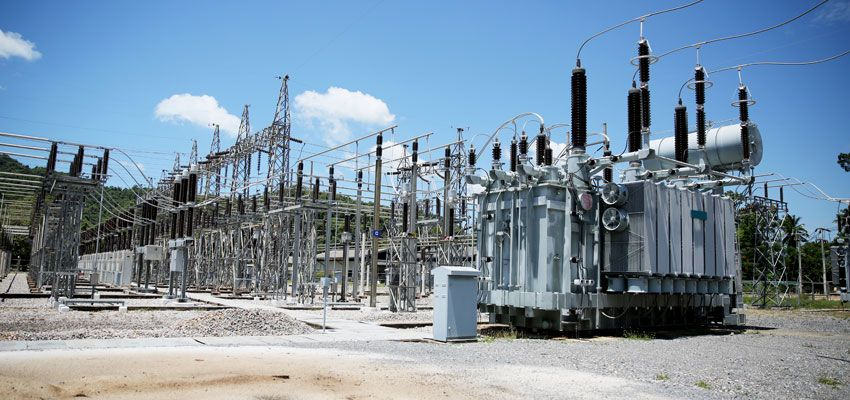
\includegraphics[width=\linewidth]{Figuras/Ch03/fig13}

		Subestação numa usina
	\end{minipage}
	\hfill
	\begin{minipage}{0.49\linewidth}
		\centering
		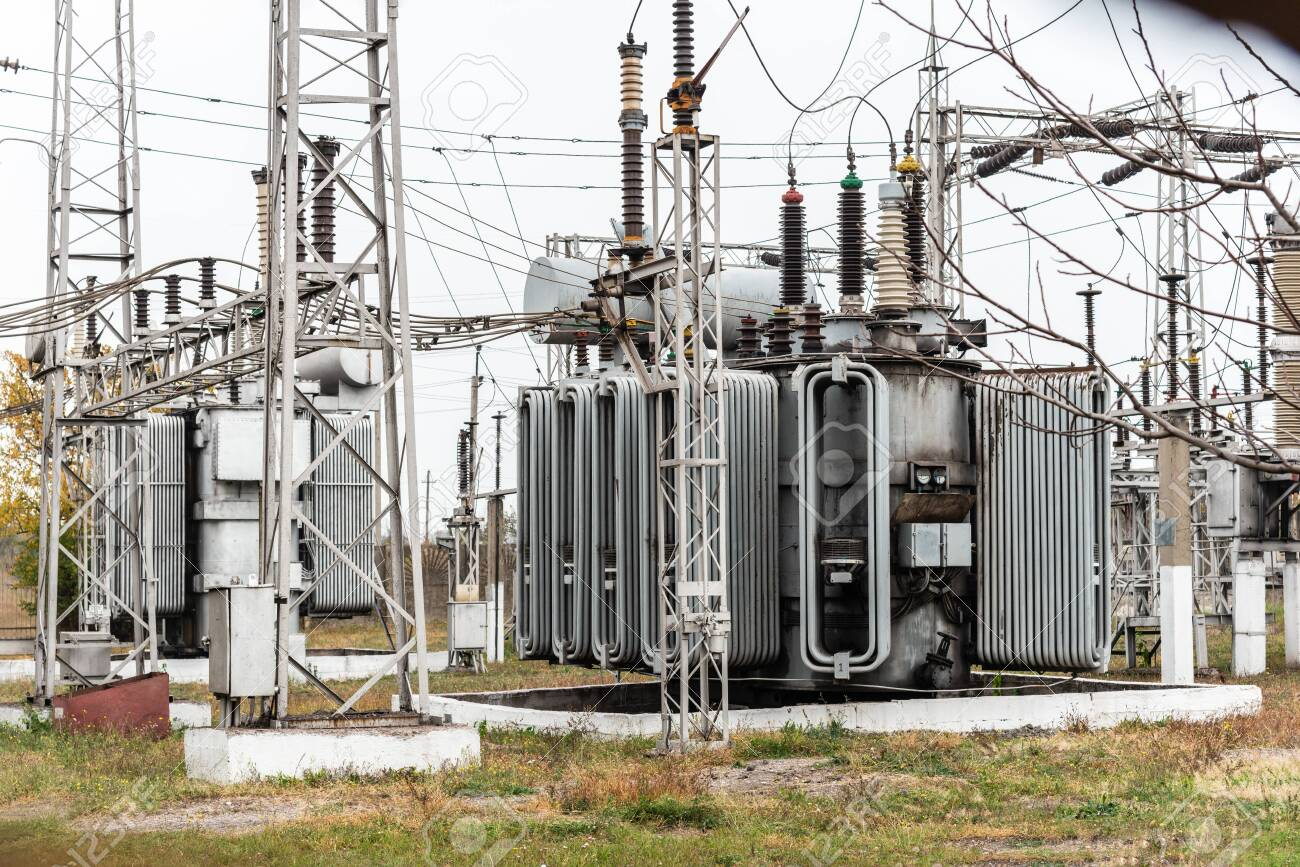
\includegraphics[width=\linewidth]{Figuras/Ch03/fig14}

		Subestação perto de uma cidade
	\end{minipage}
\end{frame}


\begin{frame}{Transmissão de energia}
	\begin{block}{Transformadores e subestações}
		\begin{itemize}
			\item Apesar de mais baixa, a tensão utilizada nas redes de distribuição \textbf{ainda não está adequada para o consumo residencial imediato}.
			\item Por isso, se faz necessária a \textbf{instalação de transformadores menores}, \textbf{instalados nos postes das ruas}, para \textbf{reduzir ainda mais a tensão} que vai para as \textbf{residências}, \textbf{estabelecimentos comerciais} e \textbf{outros locais de consumo}.
			\item É importante lembrar que o \textbf{fornecimento} de energia elétrica no Brasil é feito por meio de um \textbf{grande} e \textbf{complexo sistema de subestações} e \textbf{linhas de transmissão}, \textbf{interligadas às várias usinas de diversas empresas}. Assim, \textbf{uma cidade não recebe energia gerada por uma única usina, mas por diversas usinas} --- \textbf{hidrelétricas}, \textbf{termelétricas} ou \textbf{nucleares} --- que constituem o chamado \textbf{Sistema Interligado Nacional} (SIN).
		\end{itemize}
	\end{block}

\end{frame}


\begin{frame}{Transmissão de energia}
	\begin{block}{Transformadores e subestações}
		\begin{itemize}
			\item As tensões que circulam nos postes geralmente são de \SI{3.8}{\kilo\volt}, \SI{13.8}{\kilo\volt}, \SI{24.5}{\kilo\volt} ou \SI{34.5}{\kilo\volt}.
		\end{itemize}
	\end{block}

	\centering
	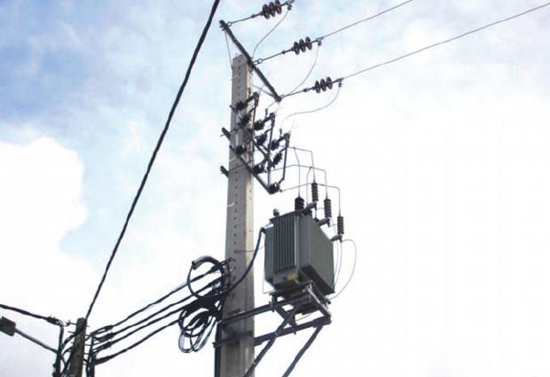
\includegraphics[height=0.65\textheight]{Figuras/Ch03/fig15}

\end{frame}


\begin{frame}{Transmissão de energia}
	\begin{block}{Transformadores e subestações}
		Além disso há vários tipos de subestações, como as
		\begin{itemize}
			\item Estação Transformadora de Transmissão – ETT

			      Converte a tensão de \textbf{geração} para uma tensão \textbf{maior} e se localiza próximo aos centros de geração.
		\end{itemize}
	\end{block}

	\centering
	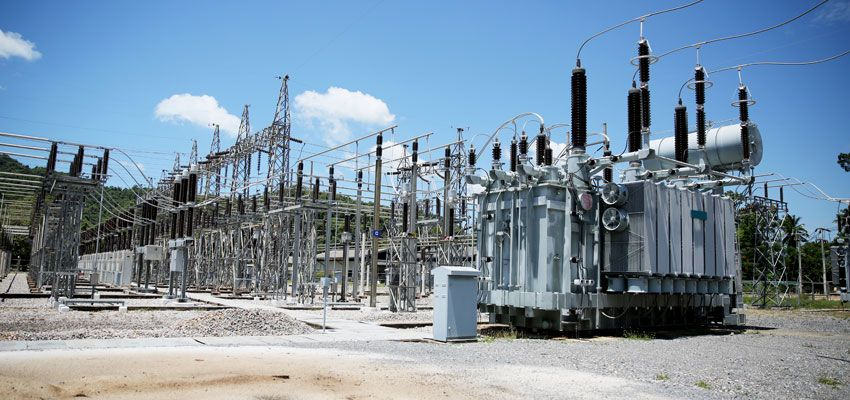
\includegraphics[width=0.85\linewidth]{Figuras/Ch03/fig13}
\end{frame}


\begin{frame}{Transmissão de energia}
	\begin{block}{Transformadores e subestações}
		\begin{itemize}
			\item Estação Transformadora de Distribuição – ETD; ou Subestação – SE

			      A subestação transformadora abaixadora converte a tensão de \textbf{transmissão} para uma tensão \textbf{menor} e se localiza próximo aos \textbf{grandes centros consumidores} ou de \textbf{fornecimento às indústrias}.
		\end{itemize}
	\end{block}

	\centering
	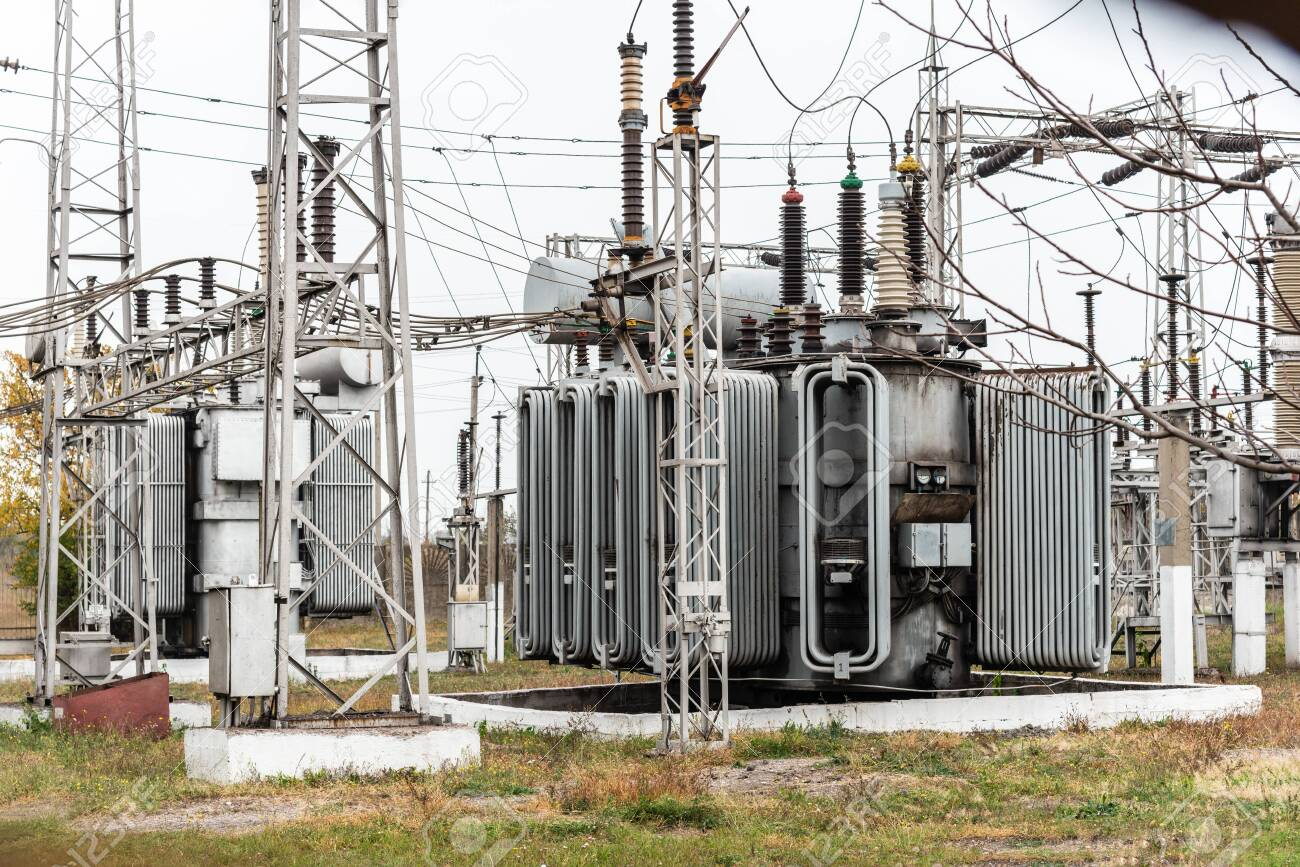
\includegraphics[width=0.55\linewidth]{Figuras/Ch03/fig14}
\end{frame}


\begin{frame}{Transmissão de energia}
	\begin{block}{Transformadores e subestações}
		\begin{itemize}
			\item Subestação Seccionadora, de Manobra ou de Chaveamento

			      É responsável por \textbf{interligar circuitos de fornecimento de energia elétrica} sob o \textbf{mesmo nível de tensão} tornando possível sua \textbf{multiplicação}, além de possibilitar o \textbf{seccionamento de circuitos}, permitindo \textbf{manobras de circuitos}.
		\end{itemize}
	\end{block}
\end{frame}


\begin{frame}{Transmissão de energia}
	\begin{block}{Transformadores e subestações}
		\begin{itemize}
			\item Subestação Interna ou Abrigada

			      Onde os equipamentos são instalados \textbf{protegidos do tempo}, podendo ser uma edificação ou câmara subterrânea. Podem consistir de cubículos metálicos, além de subestações isoladas a gás SF$ _6 $ (hexafluoreto de enxofre).
		\end{itemize}
	\end{block}

	\centering
	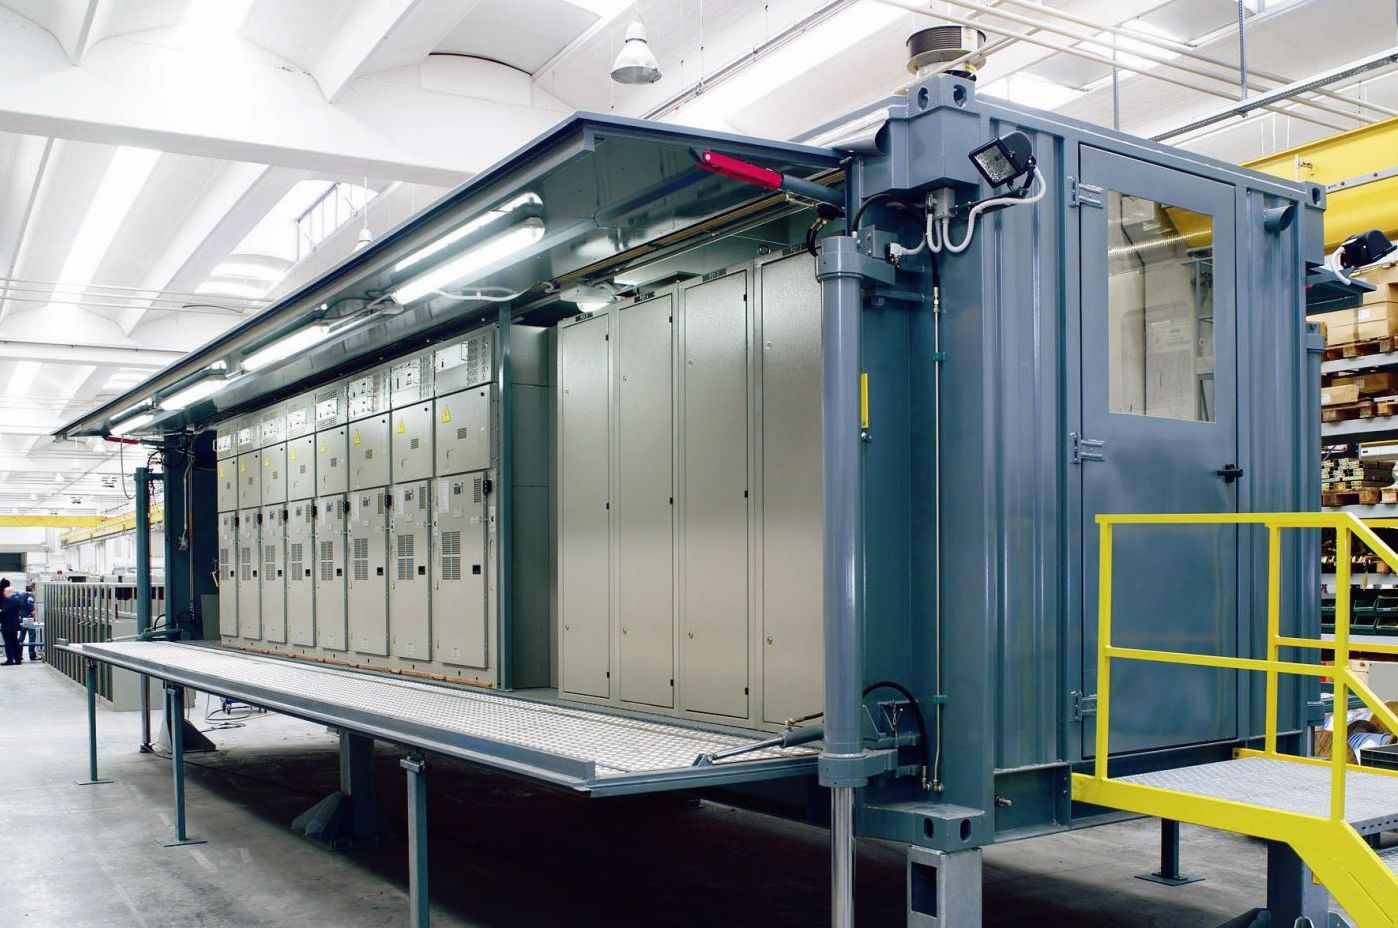
\includegraphics[width=0.55\linewidth]{Figuras/Ch03/fig17}
\end{frame}


\begin{frame}{Transmissão de energia}
	\begin{block}{Transformadores e subestações}
		\begin{itemize}
			\item Subestação Externa ou Ao Tempo

			      Os equipamentos são instalados \textbf{ao tempo} e, portanto, ficam \textbf{expostos às condições climáticas} que causam \textbf{seus desgastes e dos seus componentes}, exigindo \textbf{manutenções preventivas periódicas} para não comprometer as suas eficiências.
		\end{itemize}
	\end{block}

	\centering
	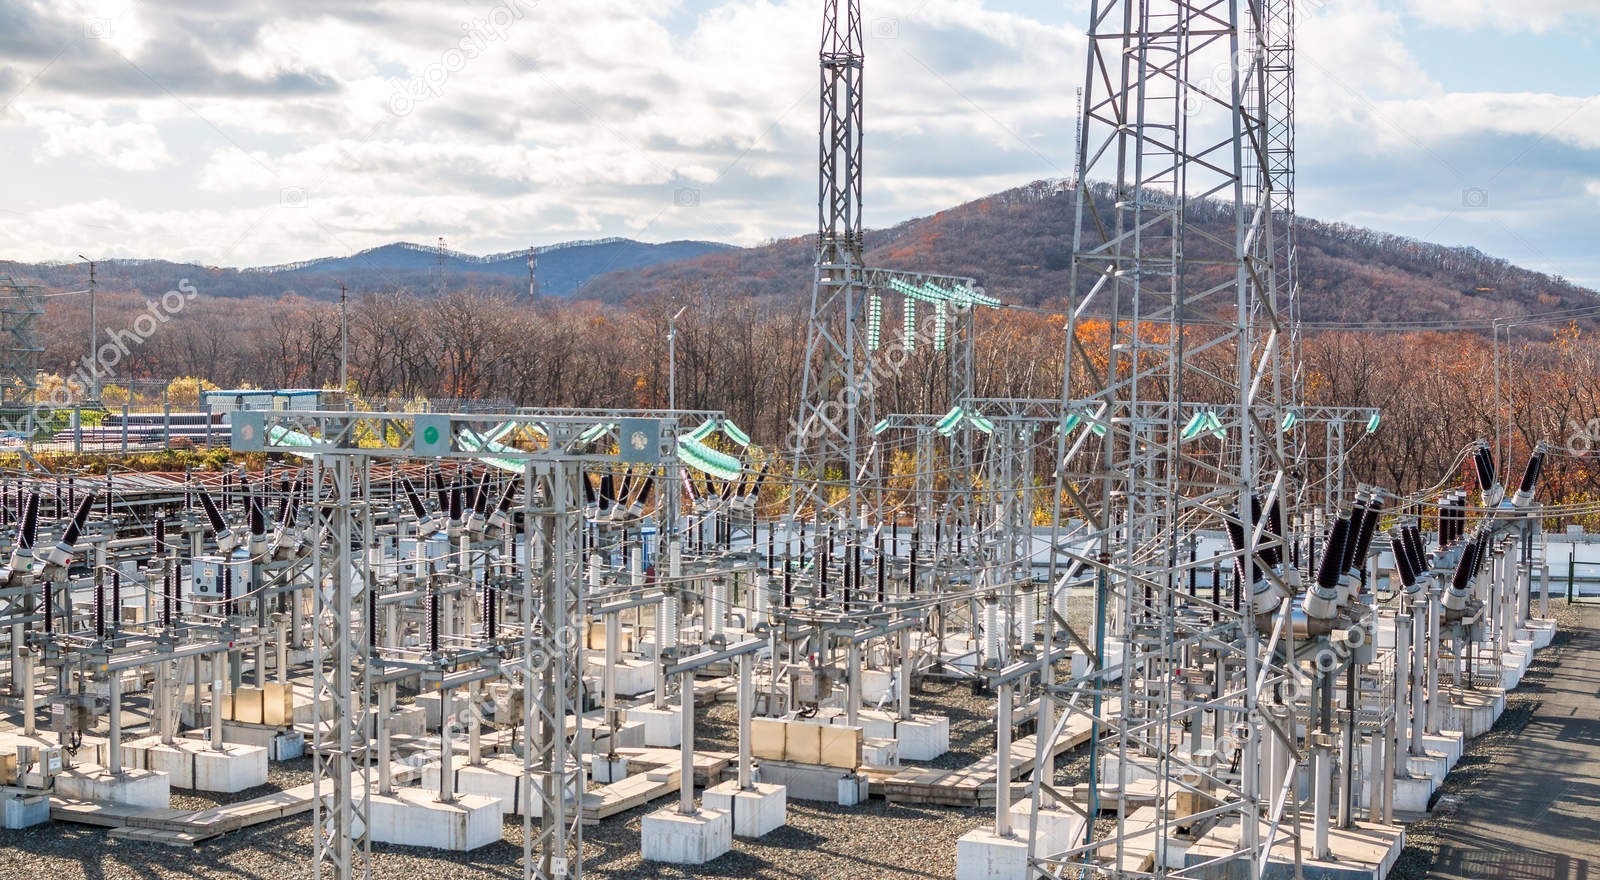
\includegraphics[width=0.7\linewidth]{Figuras/Ch03/fig16}
\end{frame}


\begin{frame}{Transmissão de energia}

	\centering
	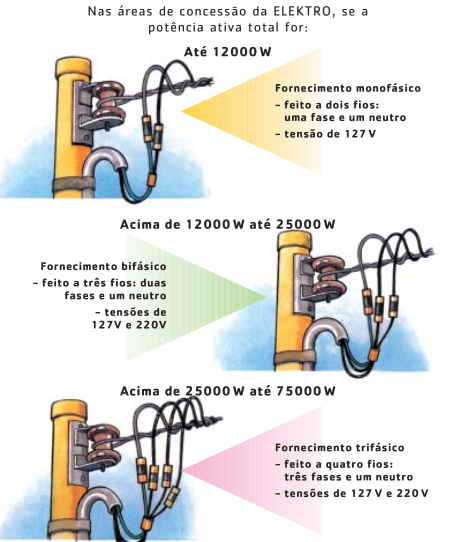
\includegraphics[height=0.9\textheight]{Figuras/Ch03/fig18}
\end{frame}


\begin{frame}{Transmissão de energia}
	\begin{minipage}{0.49\linewidth}
		\centering
		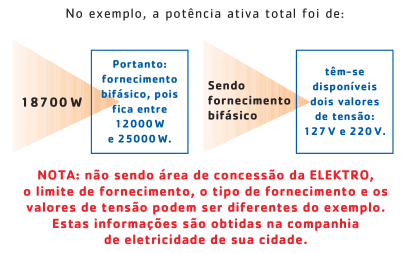
\includegraphics[width=\linewidth]{Figuras/Ch03/fig19.1}
	\end{minipage}\hfill
	\begin{minipage}{0.49\linewidth}
		\centering
		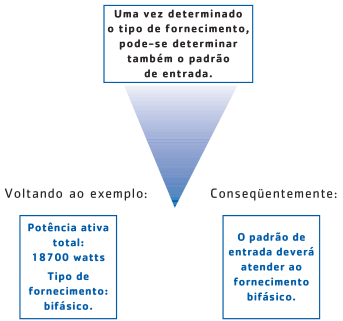
\includegraphics[width=\linewidth]{Figuras/Ch03/fig19}
	\end{minipage}

\end{frame}


\begin{frame}{Transmissão de energia}

	\centering
	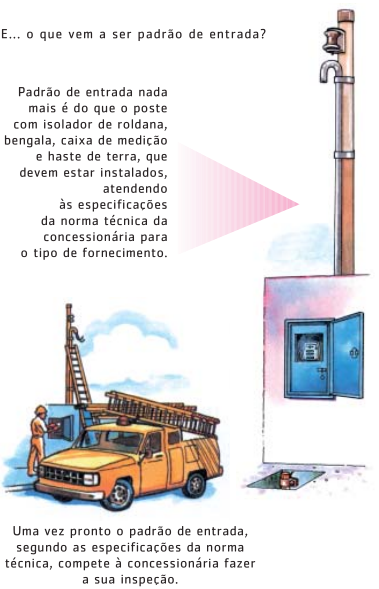
\includegraphics[height=0.9\textheight]{Figuras/Ch03/fig20}
\end{frame}


\begin{frame}{Transmissão de energia}
	\begin{minipage}{0.49\linewidth}
		\centering
		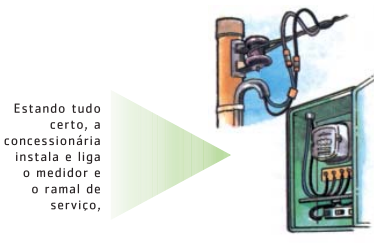
\includegraphics[width=\linewidth]{Figuras/Ch03/fig21.1}
	\end{minipage}\hfill
	\begin{minipage}{0.49\linewidth}
		\centering
		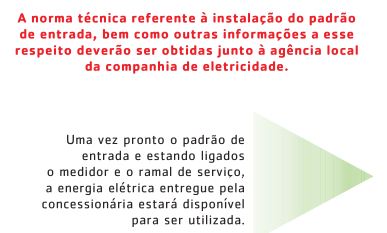
\includegraphics[width=\linewidth]{Figuras/Ch03/fig21}
	\end{minipage}

\end{frame}


\begin{frame}{Transmissão de energia}

	\centering
	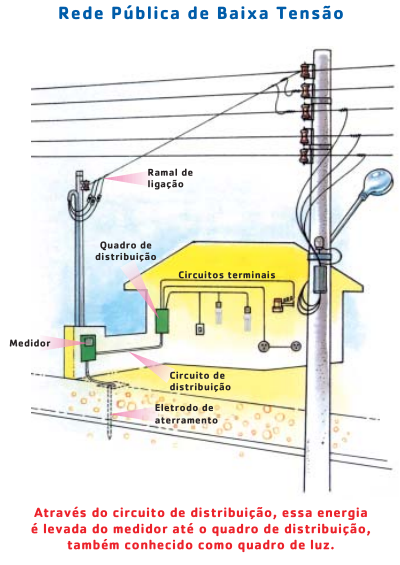
\includegraphics[height=0.9\textheight]{Figuras/Ch03/fig22}
\end{frame}


\section*{Exercícios}
\frame{
	\frametitle{Exercícios}
	\begin{block}{}
		01. Considerando o que aprendeu até agora, descreva, \textbf{com suas próprias palavras}, uma possibilidade de \textbf{abastecimento} da \textbf{demanda industrial} do \textbf{Polo Industrial de Manaus} (PIM).

		\bigskip

		02. Você sabe quais são as \textbf{principais formas} de \textbf{geração de energia} do \textbf{Brasil}? Descreva \textbf{duas} delas, \textbf{com suas próprias palavras}, complementando com o que aprendeu hoje.
	\end{block}
}

\section*{Referências}

\frame{
	\frametitle{Referências e Exercícios Complementares}
	\begin{itemize}
		\item CREDER, Hélio; Instalações Elétricas, 14ª edição, Editora LTC, Rio de Janeiro, 2004.
		\item Manual de Instalações Elétricas - Prysmian.
	\end{itemize}
	%\centering{\alert{Página 36 - \textbf{1.6.1 até 1.6.5, 1.6.17 até 1.6.19}}} \\
	%	\centering{\alert{Lista de exercícios 01}}
}